% This file is modified by Frans Oliehoek <faolieho@science.uva.nl>
% on 2005/12/18. (original file name: conference-ornate-20min.en.tex)

\documentclass[10pt]{beamer}

% Copyright 2004 by Till Tantau <tantau@users.sourceforge.net>.
%
% In principle, this file can be redistributed and/or modified under
% the terms of the GNU Public License, version 2.
%
% However, this file is supposed to be a template to be modified
% for your own needs. For this reason, if you use this file as a
% template and not specifically distribute it as part of a another
% package/program, I grant the extra permission to freely copy and
% modify this file as you see fit and even to delete this copyright
% notice. 


\mode<presentation>
{
%\usetheme{IAS_sidebar} 	% only a simple left side bar, frame-title box varies in size when using subtitles for frames.
%\usetheme{IAS_sidebar2_10pt} 	% only a simple side bar, the frame-title box has a fixed size to exactly fit a title and subtitle. For usage with 10pt font, i.e.: \documentclass[10pt]{beamer}
%\usetheme{IAS_sidebar2_11pt} 	% As above only changed to fit 11pt fonts.
%\usetheme{IAS_sidebar2_12pt} 	% As above only changed to fit 12pt fonts.
  \usetheme{IAS_sidebarNav} 	% An IAS side bar with navigation
%\usetheme{IAS_topNav}		% Only top navigation with IAS colors
%\usetheme{IAS_topNav_bottomAuthorTitle}	%Top navigation and author/title in the bottom with IAS colors
%\usetheme{IAS_topNav_leftIASbar_10pt}	% both top navigation and the IAS sidebar, the frame-title box has a fixed size to exactly fit a title and subtitle. For usage with 10pt font, i.e.: \documentclass[10pt,english
%\usetheme{IAS_topNav_leftIASbar_11pt}	% As above only changed to fit 11pt fonts.
%\usetheme{IAS_topNav_leftIASbar_12pt}	% As above only changed to fit 12pt fonts.
  \setbeamercovered{transparent}
%   % or whatever (possibly just delete it)
}


% to remove the navigation symbols:
%\setbeamertemplate{navigation symbols}{}

\usepackage[english]{babel}
% or whatever

\usepackage[latin1]{inputenc}
% or whatever



\usepackage{times}
\usepackage[T1]{fontenc}
% Or whatever. Note that the encoding and the font should match. If T1
% does not look nice, try deleting the line with the fontenc.

\usepackage{amssymb,amsbsy,amsmath,amsfonts,stmaryrd,latexsym,multirow,array}
\usepackage{movie15}
\usepackage{graphics, graphicx, color}

%\logo{\includegraphics[width=0.2\linewidth]{./figures/LogoLEMMA.pdf} }

\title[JV 2015] % (optional, use only with long paper titles)
{Projet Jeu Vid\'eo}


\author[A. Berne, X. Mapeu, G. Olivier] % (optional, use only with lots of authors)
{Antoine Berne \and Xavier Maupeu 
\and G\'eraldine Olivier
\medskip
}



%\institute[] % (optional, but mostly needed)
%{
%   \includegraphics[width=0.3\linewidth]{./figures/LogoLEMMA.pdf} \inst{1}\\
%   \medskip
%   
%   \includegraphics[width=0.3\linewidth]{./figures/LogoTotal.png} \inst{2}\\
%   \medskip
%   
%   geraldine.olivier@lemma-ing.com\\
%   olivier.allain@lemma-ing.com \\
%   mohammad.mottaghi@total.com
%    
%    
%  }
% - Use the \inst command only if there are several affiliations.
% - Keep it simple, no one is interested in your street address.

\date[Novembre 2012] % (optional, should be abbreviation of conference name)
{Jeudi 26 Novembre 2015}
% - Either use conference name or its abbreviation.
% - Not really informative to the audience, more for people (including
%   yourself) who are reading the slides online

\subject{Etude 3D de sloshing dans un s\'eparateur de phase embarqu\'e sur FPSO}
% This is only inserted into the PDF information catalog. Can be left
% out. 


% If you have a file called "university-logo-filename.xxx", where xxx
% is a graphic format that can be processed by latex or pdflatex,
% resp., then you can add a logo as follows:




% Delete this, if you do not want the table of contents to pop up at
% the beginning of each subsection:
%\AtBeginSection[]
%{
%  \begin{frame}<beamer>
%    \frametitle{Plan}
%    \tableofcontents[currentsection,currentsubsection]
%  \end{frame}
%}


\begin{document}

\begin{frame}[plain]
  \titlepage
  
\end{frame}

%\begin{frame}
%  \frametitle{Outline}
%  \tableofcontents
%\end{frame}



\begin{frame}{Principe du jeu: capture de zones}

\begin{center}
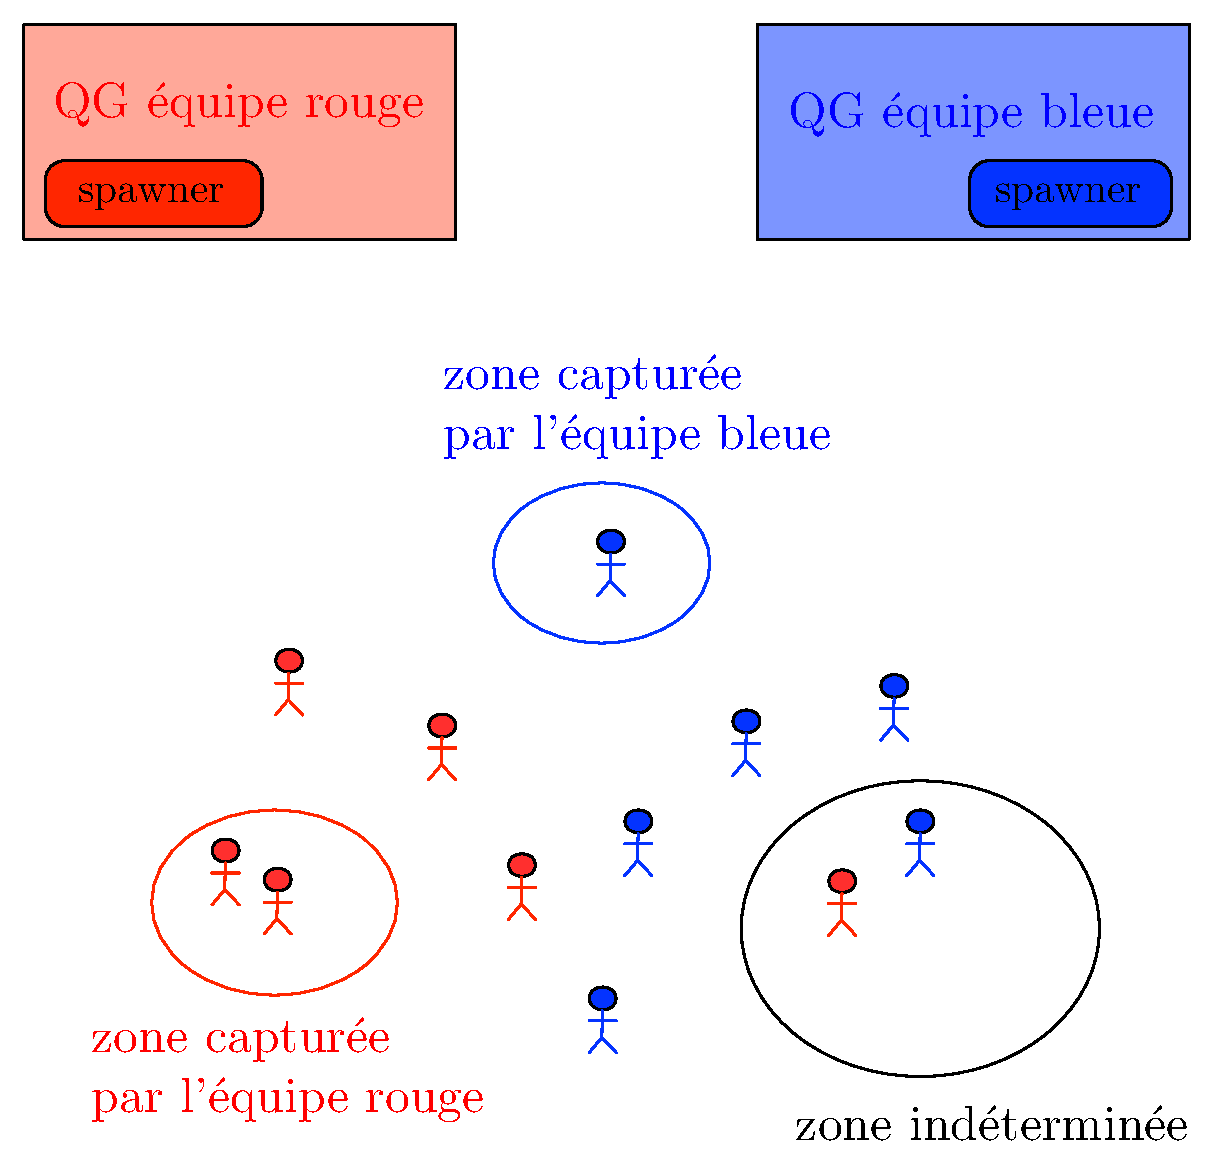
\includegraphics[width=0.75\linewidth]{./zones.pdf}
\end{center}
\end{frame}



\begin{frame}{Principe du jeu: Actions}

\begin{itemize}
\item La partie dure un temps fix\'e. 

\medskip


\item L'\'equipe gagnante est celle qui a le plus de points \`a l'issue de la partie.

\medskip


\item Le joueur contr\^ole un seul personnage de son \'equipe.

\medskip


\item Ses co-\'equipiers et ses adversaires sont g\'er\'es par l'IA.

\medskip

\item Le joueur peut donner des ordres simples \`a ses co-\'equipiers:
\begin{itemize}
\item Aidez-moi!
\item A l'attaque!
\item En d\'efense!
\end{itemize}

\end{itemize}

\end{frame}

\begin{frame}{Principe du jeu: Actions}

\begin{block}{Trois types des personnages}
\begin{description}
\item[Tireur:] peut tuer les adversaires en un coup 
\item[Protecteur:] prot\`ege un co\'equipier en difficult\'e 
\item[Ing\'enieur:] construit des obstacles pour emp\^echer l'adversaire d'entrer dans une zone.
\end{description}
\end{block}

\bigskip

\begin{block}{Pour tous les personnages}
\begin{itemize}
\item capacit\'e \`a d\'etruire les obsctales
\item \`a enlever des points de vie aux adversaires
\item utilisation de grenades
\end{itemize}
\end{block}

\end{frame}

\begin{frame}{Principe du jeu: Capacit\'es des personnages}
\begin{tabular}{|c||c|c|c|}
\hline
&&&\\
					& Tireur & Ing\'enieur & Protecteur \\
&&&\\
\hline
&&&\\
Rapidit\'e 				& +        & -                 & --               \\
&&&\\
Points de vie			& -         & +                &++               \\
&&&\\
Destruction d'obstacles	& -         & +                & ++               \\
&&&\\
Capacit\'e d'attaque		& ++      & -                 & -                  \\
&&&\\
\hline
\end{tabular}

\end{frame}

\begin{frame}{D\'eveloppement}

\begin{block}{Outils}
\begin{itemize}
\item  Unity3D
\item GitHub
\end{itemize}
\end{block}

\begin{block}{Travail r\'ealis\'e}
\begin{itemize}
\item NavMesh
 \item Prefab Zone
 \item Prefab Minimap
 \item Prefab Brouillard de Guerre
 \item Architecture de classes TeamsManager, Player
\end{itemize}
\end{block}
\end{frame}

\begin{frame}{D\'eveloppement}
\begin{block}{Travail restant}
\begin{itemize}
 \item IA pour chaque type de personnage (+++)
 \item Comptage des points
 \item Utilisation et param\'etrage du Game Play (+++)
 \item Visuel
 \item Deux joueurs, r\'eseau (si temps restant)
\end{itemize}
\end{block}

\end{frame}

\end{document}



